\documentclass[a4paper]{article}
\usepackage{natbib,amsmath,geometry,float}
\geometry{margin=1in}
\restylefloat{table}

\title{\texttt{exactLoglinTest}: A Program for Monte Carlo Conditional
Analysis of Log-linear Models} 
\author{Brian S. Caffo}

%\newcommand{\eqref}[1]{(\ref{#1})}
\newcommand{\mcexact}{\texttt{mcexact} }

\usepackage{/home/bcaffo/local/R-lr/share/texmf/Sweave}
\begin{document} 
\maketitle 

Nuisance parameters are parameters that are not of direct interest to
the inferential question in hand. In a frequentist or likelihood
paradigm, a common tool for eliminating nuisance parameters is to
condition on their sufficient statistics. The same technique is useful
(though rarely used) in a Bayesian settings, as it eliminates the need
to put priors on nuisance parameters.

For log-linear models, conditional analysis suffers from two main drawbacks.
\begin{enumerate}
\item The set of lattice points contained in the conditional distribution is difficult to manage, 
      computationally or analytically.
\item The sufficient statistics for the nuisance parameters are not ancillary to the 
      parameters of interest.
\end{enumerate}
In this manuscript we address only the first drawback using \texttt{exactLoglinTest}.

\section{The Problem} 

The observed data, $y = (y_1, \ldots, y_n)$, are modeled as Poisson
counts with a means, $\mu = (\mu_1,\ldots,\mu_n)$, satisfying $$ \log
\mu = x \beta $$ under the null hypothesis. Here $x$ is a full rank
$n\times p$ design matrix. It is easily shown that the sufficient
statistics for $\beta$ under the null hypothesis are $x^t y$, where a
superscript $t$ denotes a transpose. Let $h$ be a test statistic of
interest where larger values of $h$ support the alternative
hypothesis. Two examples are the Pearson Chi-Squared statistic and the
deviance. An exact test relative to $h$ can be performed via the
conditional P-value
$$
\mbox{Prob}\{h(y) \geq h(y_{obs}) | x^t y = x^t y_{obs}\} = \sum_{\{y
\in \Gamma\}} \frac{I\{h(y) \geq h(y_{obs})\}}{C \prod y_i!}  
$$ 
where $y_{obs}$ is the observed table, $C$ is a normalizing
constant and $\Gamma = \{y | x^t y = x^t y_{obs}\}$  (often referred
to as the reference set).

The term ``exact'' is used to refer to tests that guarantee the
nominal type I error rate unconditionally. Thus a test that never
rejects the null hypothesis is technically exact in any
situation. Therefore, exactness is not in itself a sufficient
condition for a test to be acceptable.  Moreover, this example (never
rejecting) is particularly relevant in our setting because $\Gamma$
may contain one or few elements. Hence the conditional P-value will be
exactly or near one regardless of the evidence in the data vis-a-vis
the two hypotheses.  However, it is also the case that the
conservative conditional tests can produce P-values that are smaller
than those calculated via Chi-squared approximations (see Subsection
\ref{path} for an example).

\subsection{Binomial Calculations}
\label{sec:binom}
Conditional inference for Poisson log-linear models contains
conditional inference for binomial-logit models as a special
case. Consider a binomial logit models of the form, $b_i \sim
\mbox{Bin}(n_i,p_i)$ for $i=1,\ldots,k$ and
\begin{equation}
\label{logitmodel}
 \mbox{logit}(p_{i}) = z_i \gamma + x_i' \beta,
\end{equation}
where $\gamma$ is a scalar and $\beta$ is a $p$ dimensional vector.
Frequently, $x_i'$ contains only a strata indicator and an intercept
term. In this case conditioning on the sufficient statistic for
$\beta$ results in standard conditional logistic regression. For this
purpose, we suggest the \texttt{coxph} function as described in
\cite{vr:2002}. Instead we consider the more general case where
$\beta$ is arbitrary vector of nuisance parameters.  However, the
reader should again be warned that the loss of information from
conditioning can sometimes be quite severe in these problems and hence
produce useless results.


Consider testing $H_0 \gamma = 0$ versus some alternative.
The following model model is equivalent to the null modell for
\eqref{logitmodel}:
\begin{equation}
\label{eq:poisson}
y_{ij} \sim \mbox{Poisson}(\mu_{ij}) 
\hspace{.3in} 
\mbox{log}(\mu_{i1}) = \alpha_i + x_i' \beta
\hspace{.3in} 
\mbox{log}(\mu_{i2}) = \alpha_i,
\end{equation}
for $j=1,2$ and $i=1,\ldots,k$.  The sufficient statistics for the
$\alpha_i$ are $y_{i1} + y_{i2} = y_{i+}$. Then it is easy to show
that the conditional distribution of $y_{i1} | y_{i+}$ is precisely
the model given by \eqref{logitmodel} where
\begin{eqnarray*}
  p_i & = &\mu_{i1} / \mu_{i+} \\
  b_i & = & y_{i1} \\
  n_i & = & y_{i+}.
\end{eqnarray*}
Therefore, conditioning out the nuisance parameters $\{\alpha_i\}$ and
$\beta$ for the Poisson log-linear model yields exactly the same
(null) conditional distribution as conditioning out $\beta$ in model
\eqref{logitmodel}.  Furthermore, this exercise indicates exactly how
to perform the calculations, which is useful since \texttt{exactLoglinTest} only
accepts models in the form of Poisson log-linear models.

Currently \texttt{exactLoglinTest} is useful for tests of $\gamma = 0$. With
modifications, the central ideas could be used to calculate a Monte
Carlo estimate of the conditional likelihood for $\gamma$. (It is
possible to use \texttt{exactLoglinTest} as is for this purpose. However, we have had
mixed success in this endeavor and it is best avoided due to numerical
instability.)

\section{\texttt{exactLoglinTest}} 
The software \texttt{exactLoglinTest} is an implementation of the algorithms presented
in \cite{booth:butler:1999} and \cite{caffo:booth:2000} using the R open source
programming language \cite{ihaka:gent}.  At the heart
of both algorithms is a sequentially generated rounded normal
approximation to the conditional distribution. We refer the reader
to those papers for a more complete description.

You can obtain a copy of \texttt{exactLoglinTest} at the Comprehensive R Archive Network,
\begin{verbatim}
http://cran.R-project.org
\end{verbatim}
Also included in the CRAN documentation is a noweb version of this
document.  Please refer to the ``An Introduction to R'' manual,
included with your R distribution, for details on how to install
packages. Assuming it is installed, one can load
\texttt{exactLoglinTest} with
\begin{Schunk}
\begin{Sinput}
> library(exactLoglinTest)
> set.seed(1)
\end{Sinput}
\end{Schunk}
Here, the optional argument \texttt{lib.loc} is necessary if the
package has been installed into one of the paths that R automatically
checks. We remind the reader that is a good idea to set the random
number seed to a specific value, so that results can be reproduced.

\section{Examples}
\subsection{Residency Data}
Assuming \texttt{exactLoglinTest} has been properly installed, the residency data can
be obtained by the command
\begin{Schunk}
\begin{Sinput}
> data(residence.dat)
\end{Sinput}
\end{Schunk}
This data is a 4$\times$4 table of subjects' residence in 1985 by
their residence in 1980; Table \ref{tab:res} displays the data in a
tabular format.  The extra term, \texttt{sym.pair}, in the data frame
is used to fit a quasi-symmetry model. (For details on the
quasi-symmetry model see \cite{agre:1990}.)  A Monte Carlo goodness of
fit test of quasi-symmetry versus a saturated model involves the
following command
\begin{Schunk}
\begin{Sinput}
> resid.mcx <- mcexact(y ~ res.1985 + res.1980 + factor(sym.pair), 
+     data = residence.dat, nosim = 10^2, maxiter = 10^4)
> resid.mcx
\end{Sinput}
\begin{Soutput}
                deviance    Pearson
observed.stat 2.98596233 2.98198696
pvalue        0.46311695 0.46311695
mcse          0.03679595 0.03679595
\end{Soutput}
\end{Schunk}

The default method used for sampling is the importance sampling
algorithm of \cite{booth:butler:1999}. Because this method rejects
simulated table with negative entries, the number of desired
simulations \texttt{nosim} may not be met in \texttt{maxiter}
iterations and no warning is issued if this occurs. 

The returned object is a list storing the results of the Monte Carlo
simulation as well as all of the relevant information necessary to
restart the simulation.  More information can be obtained with
\texttt{summary}
\begin{Schunk}
\begin{Sinput}
> summary(resid.mcx)
\end{Sinput}
\begin{Soutput}
Number of iterations       =  100 
T degrees of freedom       =  3 
Number of counts           =  16 
df                         =  3 
Next update has nosim      =  100 
Next update has maxiter    =  10000 
Proportion of valid tables =  1 

                deviance    Pearson
observed.stat 2.98596233 2.98198696
pvalue        0.46311695 0.46311695
mcse          0.03679595 0.03679595
\end{Soutput}
\end{Schunk}
The $t$ degrees of freedom refers to degrees of freedom used as a
tuning parameter within the algorithm while the \texttt{df} refers to
the model degrees of freedom. In this case, the Monte Carlo standard
error, \texttt{mcse}, is too large. The simulation can be restarted
using \texttt{update}
\begin{Schunk}
\begin{Sinput}
> resid.mcx <- update(resid.mcx, nosim = 10^4, maxiter = 10^6)
> resid.mcx
\end{Sinput}
\begin{Soutput}
                 deviance     Pearson
observed.stat 2.985962330 2.981986964
pvalue        0.397222805 0.396772921
mcse          0.003596126 0.003594809
\end{Soutput}
\end{Schunk}
Here \texttt{nosim} is the number of additional simulations desired
and \texttt{maxiter} is maximum number of iterations allowed.  It is
important to note that \texttt{update} can only resume the simulation
with changes with a new Monte Carlo sample size. It does not allow
users to change the model formulation; one must rerun \mcexact
independently to do that.

This example illustrates the point that the underlying algorithms are
very efficient when the cell counts are large. Of course, when this is
the case, the large sample approximations are nearly identical to the
conditional results
\begin{Schunk}
\begin{Sinput}
> pchisq(c(2.986, 2.982), 3, lower.tail = FALSE)
\end{Sinput}
\begin{Soutput}
[1] 0.3937887 0.3944088
\end{Soutput}
\end{Schunk}

\subsection{Pathologists' Tumor Ratings}
\label{path}
The following example is interesting in that the large sample results
differ drastically from the conditional results. Moreover, the
conditional results are {\em less} conservative. 
The data from given in Table \ref{tab:path} cross clasify two pathologists'
tumor ratings and can be obtained in R with the command
\begin{Schunk}
\begin{Sinput}
> data(pathologist.dat)
\end{Sinput}
\end{Schunk}
A uniform association model accounts for the ordinal nature of the
ratings by assigning ordinal scores to the ratings
\citep[see][]{agre:1990}. We test the uniform
association model against the saturated model with
\begin{Schunk}
\begin{Sinput}
> path.mcx <- mcexact(y ~ factor(A) + factor(B) + I(A * B), data = pathologist.dat, 
+     nosim = 10^4, maxiter = 10^4)
> summary(path.mcx)
\end{Sinput}
\begin{Soutput}
Number of iterations       =  4444 
T degrees of freedom       =  3 
Number of counts           =  25 
df                         =  15 
Next update has nosim      =  10000 
Next update has maxiter    =  10000 
Proportion of valid tables =  0.4444 

                  deviance      Pearson
observed.stat 16.214534925 14.729278917
pvalue         0.037393837  0.126297722
mcse           0.001194588  0.002990041
\end{Soutput}
\end{Schunk}
It is worth comparing these results to the asymptotic Chi-squared 
results
\begin{Schunk}
\begin{Sinput}
> pchisq(c(16.214, 14.729), 15, lower.tail = FALSE)
\end{Sinput}
\begin{Soutput}
[1] 0.3679734 0.4711083
\end{Soutput}
\end{Schunk}

\subsection{Alligator Food Choice Data Using MCMC}
In this example we illustrate the algorithm
from\cite{caffo:booth:2000} using the data and Poisson log-linear
model from the alligator food choice data shown in Table
\ref{tab:alli}.  This data set and model is a good choice for MCMC as
the percent of valid tables generated using \texttt{method = "bab"} is
very small, less than 1\% of the tables simulated. It is often the
case that the MCMC algorithm will be preferable when the table is
large and/or sparse.  Of course, using MCMC introduces further
complications in reliably running and using the output of the
algorithm.

The algorithm from \cite{caffo:booth:2000} uses local moves to reduce
the number of tables with negative entries that the chain produces.
You can use this method with \texttt{method = "cab"} of \mcexact. The
parameter \texttt{p} of \mcexact represents the average proportion of table
entries left fixed. So a chain with \texttt{p=.9} will leave most of
the table entries fixed from one iteration to the next. A high value
of \texttt{p} will often result in a high proportion of valid
(non-negative) simulated tables. Unfortunately a large of a value of
\texttt{p} can cause the chain to mix slowly because the tables will
be very similar from one iteration to the next. However, it is also
sometimes the case that a small value of \texttt{p} will produce too
many tables with negative entries. Hence the Metropolis/Hastings/Green
algorithm will stay at the current table for long periods and again
result in a slowly mixing chain.  It is also worth mentioning that
despite the fact that the chains will be theoretically irreducible for
any value of \texttt{p} (other than 1), it is possible for chains to
be practically (numerically) reducible. 

The program allows for the option to save the chain goodness of fit
statistics,\texttt{savechain = TRUE}, so that some initial tinkering
can be performed.  (If using impartance sampling, i.e. \texttt{method =
"bab"}, then \texttt{savechain} saves both the statistic values and
the importance weights on the log scale.) Here we save the chain of goodness
of fit statistics for the alligator food choice data.
\begin{Schunk}
\begin{Sinput}
> data(alligator.dat)
> alligator.mcx <- mcexact(y ~ (lake + gender + size) * food + 
+     lake * gender * size, data = alligator.dat, nosim = 10^3, 
+     method = "cab", savechain = TRUE, batchsize = 100, p = 0.75)
> summary(alligator.mcx)
\end{Sinput}
\begin{Soutput}
Number of iterations       =  1000 
T degrees of freedom       =  3 
Number of counts           =  80 
df                         =  40 
Number of batches          =  10 
Batchsize                  =  100 
Next update has nosim      =  1000 
Proportion of valid tables =  0.196 

                 deviance     Pearson
observed.stat 50.26368862 52.56768703
pvalue         0.20000000  0.24900000
mcse           0.07231182  0.08921827
\end{Soutput}
\end{Schunk}
The chain of goodness of fit statistics are saved in
\texttt{alligator.mcx}\$\texttt{chain}. Note that the saved chain is
discarded if the simulations are resumed with \texttt{update}, even if
\texttt{savechain = T} when the simulation is resumed.

We would want to look at the autocorrelation function of the goodness
of fit statistics.
\begin{center}
\begin{Schunk}
\begin{Sinput}
> par(mfrow = c(2, 1))
> acf(alligator.mcx$chain[, 1])
> acf(alligator.mcx$chain[, 2])
\end{Sinput}
\end{Schunk}
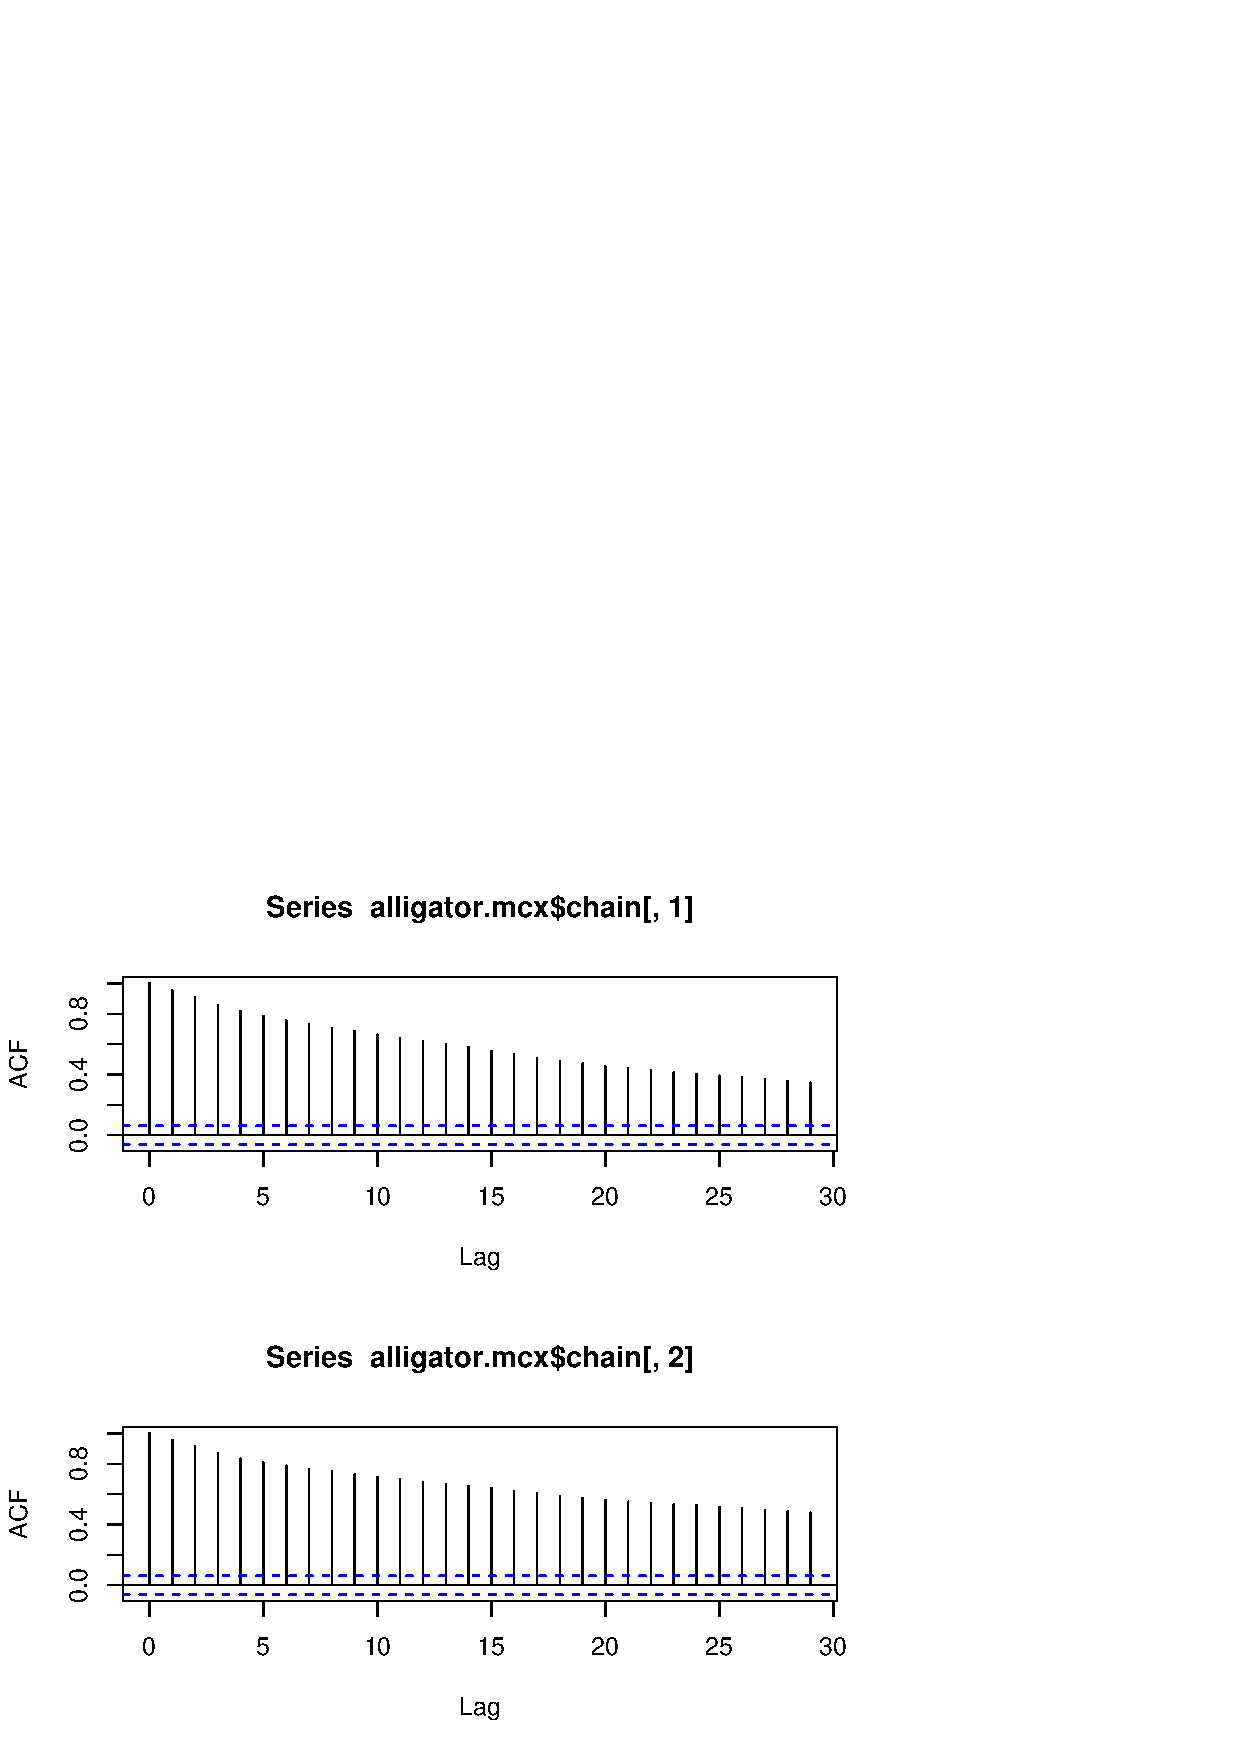
\includegraphics{exactLoglinTest-011}
\end{center}
It is also usually useful to look at the chain of P-values
\begin{center}
\begin{Schunk}
\begin{Sinput}
> dev.p <- cumsum(alligator.mcx$chain[, 1] >= alligator.mcx$dobs[1])/(1:alligator.mcx$nosim)
> pearson.p <- cumsum(alligator.mcx$chain[, 1] >= alligator.mcx$dobs[1])/(1:alligator.mcx$nosim)
> par(mfrow = c(2, 1))
> plot(dev.p, type = "l", ylab = "P-value", xlab = "iteration")
> title("Deviance P-value by iteration")
> plot(pearson.p, type = "l", ylab = "P-value", xlab = "iteration")
> title("Pearson P-value by iteration")
\end{Sinput}
\end{Schunk}
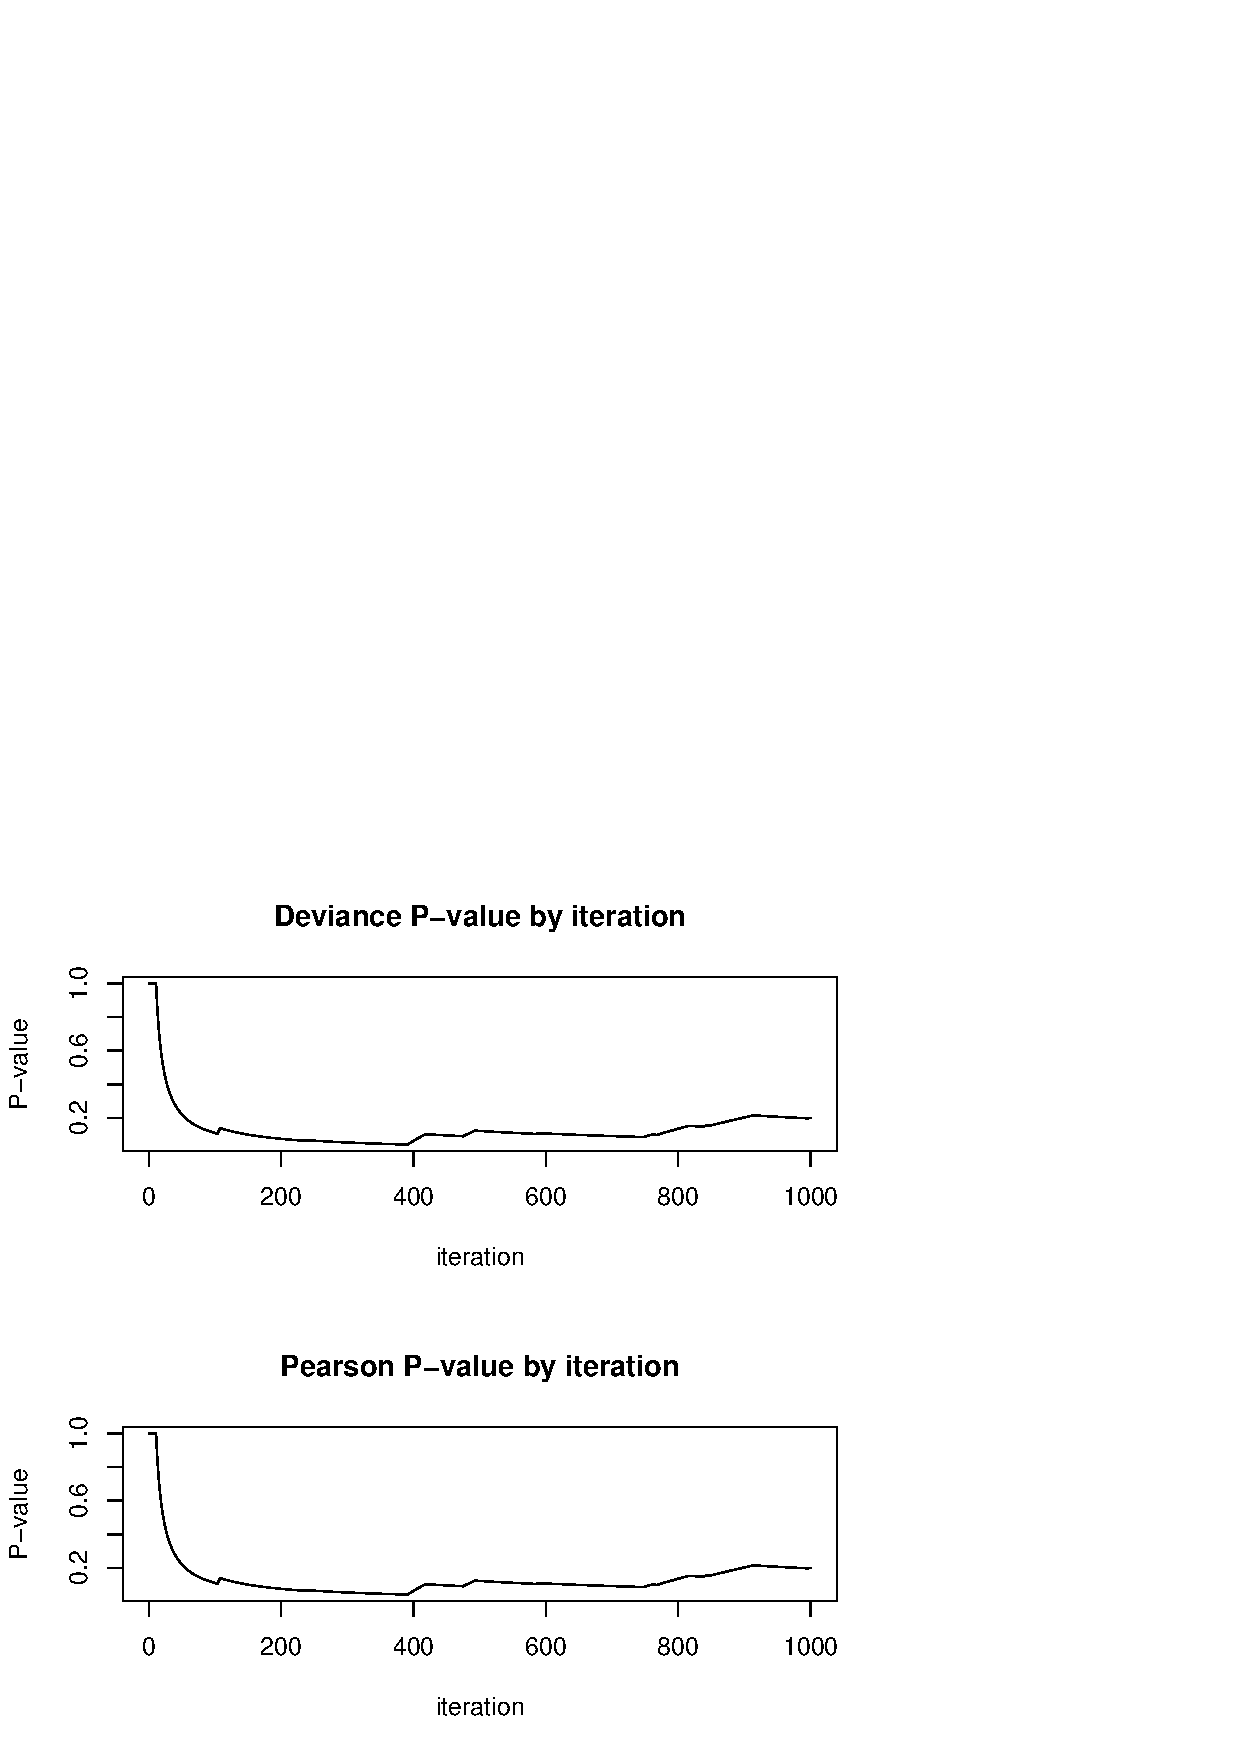
\includegraphics{exactLoglinTest-012}
\end{center}
Note that there is an extremely slow decay in the autocorrelations of
the chain of goodness of fit statistics and the P-values for the two
statistics do not seem to have converged. Therefore, we should should
execute a much longer run. Also, \mcexact uses batch means to estimate
the Monte Carlo error, and so this suggest we should use very large
batch sizes. 

While on the subject of batch sizes, note that \mcexact does not
require the total number of simulations to be a multiple of the batch
size. If the algorithm terminates in the middle of completing a batch,
that batch is not used in the P-value calculations. However, the
simulations are not wasted if the algorithm is resumed with
\texttt{update}.

One large final run of this data discarding all of the initial
tinkering could be performed by setting \texttt{flush = TRUE} as an
argument to \texttt{update}.  Here, \texttt{flush = TRUE}, tells
\texttt{update} to throw out all of the data used in the initial
tinkering, except that it starts the new chain from the final table
from the initial runs. This is a harmless way to burn the chain in
while you are tinkering with it.  Of course, the chain can be
restarted at the default starting value, the observed data, by simply
rerunning \mcexact.

\section{Application to Disclosure Limitation}
Though there are certainly more rigorous procedures available
\citep[see][]{dobra}, \texttt{exactLoglinTest} is a useful tool for exploring
disclosure limitation in contingency tables.  Consider the Czech Auto
Worker's data given in Table \ref{tab:czech}. Suppose a researcher is
concerned about the potential disclosure risk of releasing all two-way
marginals from this table. The following code will load the Czech auto
worker data into a data frame:
\begin{Schunk}
\begin{Sinput}
> data(czech.dat)
\end{Sinput}
\end{Schunk}

We will explore disclosure limitation by simulating tables from the
hypergeometric distribution obtained by conditioning on all two way
margins. However, we would like to save all of the simulated table
entries, not just the deviance and Pearson statistics. This could be
accomplished by changing the argument \texttt{stat} of \mcexact to an
appropriate statistic. However, the function
\texttt{simulate.conditional} performs this simulation for us. This
function returns the simulated tables in a matrix with each row being
a complete simulated table.

Below we run the chain
\begin{Schunk}
\begin{Sinput}
> chain <- simulate.conditional(y ~ (A + B + C + D + E + F)^2, 
+     data = czech.dat, method = "cab", nosim = 10^3, p = 0.4)
\end{Sinput}
\end{Schunk}
Now, \texttt{chain} is a matrix where each row is a complete
simulated table satisfying the two-way margins of the original
table. We were particularly concerned with cells 39, 48, and 55 which
contained only one, two and two individuals in the observed data 
respectively. Consider the proportion of tables which have greater 
than 0 but fewer than three individuals
\begin{Schunk}
\begin{Sinput}
> mean(chain[, 39] > 0 & chain[, 39] < 3)
\end{Sinput}
\begin{Soutput}
[1] 0.447
\end{Soutput}
\begin{Sinput}
> mean(chain[, 48] > 0 & chain[, 58] < 3)
\end{Sinput}
\begin{Soutput}
[1] 0.357
\end{Soutput}
\begin{Sinput}
> mean(chain[, 55] > 0 & chain[, 55] < 3)
\end{Sinput}
\begin{Soutput}
[1] 0.544
\end{Soutput}
\end{Schunk}

We used the model in question because this model fixes all two-way
margins.  However, that model need not fit the data well (in fact, it
doesn't). Therefore, in addition to simulating from the hypergeometric
density, a user would likely also want to simulate from other
densities, such as a uniform distribution on tables with these
margins. Though the normal approximations for \texttt{exactLoglinTest} 
were tailored specifically to the hypergeometric density, it 
allows for other target distributions. Here the density must be specified 
on the log scale up to a constant. Since a uniform density is simply a 
constant, we use a function that just returns 0 in the \texttt{dens = }
option.
\begin{Schunk}
\begin{Sinput}
> chain2 <- simulate.conditional(y ~ (A + B + C + D + E + F)^2, 
+     data = czech.dat, method = "cab", nosim = 10^3, p = 0.4, 
+     dens = function(y) 0)
> mean(chain2[, 39] > 0 & chain2[, 39] < 3)
\end{Sinput}
\begin{Soutput}
[1] 0.054
\end{Soutput}
\begin{Sinput}
> mean(chain2[, 48] > 0 & chain2[, 58] < 3)
\end{Sinput}
\begin{Soutput}
[1] 0.99
\end{Soutput}
\begin{Sinput}
> mean(chain2[, 55] > 0 & chain2[, 55] < 3)
\end{Sinput}
\begin{Soutput}
[1] 0.95
\end{Soutput}
\end{Schunk}

Both simulations suggest that there are plenty of tables with higher
counts than the observed counts for cells 39, 48 and 55. Hence the
disclosure risk in releasing the two-way marginals seems minimal.
However, it should be reiterated that this example is given only to
illustrate how to obtain simulated tables from
\texttt{exactLoglinTest}.

\subsection{Exact Score Test for Binomial Counts}
The data given in \ref{tab:titanic} are obtained from the Cytel (the makers
of StatXact) web site\footnote{http://www.cytel.com/}. The data cross-classify the
survival of the Titanic passengers by class, gender and age. You can
obtain the data with
\begin{Schunk}
\begin{Sinput}
> data(titanic.dat)
> titanic.dat$alpha <- rep(1:16, 2)
\end{Sinput}
\end{Schunk}
The varianble \texttt{alpha} is added to correspond to the $\alpha_i$
terms from \eqref{eq:poisson}.

Following the analysis done at the Cytel web site, we view each
person's survival as a binary outcome. We use a model where a person's
age, gender and class are additive effects on the logit scale. 
The corresponding Poisson log-linear model has model formula
\begin{Schunk}
\begin{Soutput}
y ~ (factor(class) + factor(age) + factor(sex)) : factor(surv) + factor(surv) + factor(alpha)
\end{Soutput}
\end{Schunk}

 Consider the gender effect in specific. To calculate an exact
P-value we use \texttt{simulate.conditional} to
simulate tables conditioning on all of the parameters, setting the  
\text{factor(surv) : factor(sex)} nteraction to 0.
\begin{Schunk}
\begin{Sinput}
> chain <- simulate.conditional(y ~ factor(surv) + (factor(class) + 
+     factor(age)):factor(surv) + factor(alpha), dat = titanic.dat, 
+     nosim = 10^4, method = "cab", p = 0.1)
\end{Sinput}
\end{Schunk}

A P-value for a score test of $H_0 : \gamma = 0$ versus $H_a : \gamma
< 0$ simply counts the proportion of tables with sufficient statistic
for $\gamma$ is smaller than the observed value. Using the notation
from \eqref{eq:poisson} the sufficient statistic for $\gamma$ is
$s_\gamma = \sum_i z_i y_i \equiv z' y$. We calculate the chain of
sufficient statistics and the observed sufficient statistic below.
\begin{Schunk}
\begin{Sinput}
> z <- titanic.dat$sex * titanic.dat$surv
> sgamma <- chain %*% z
> sgamma.obs <- titanic.dat$y %*% z
> mean(sgamma <= sgamma.obs[1])
\end{Sinput}
\begin{Soutput}
[1] 2e-04
\end{Soutput}
\end{Schunk}
Apparently, few of the simulated tables have sufficient statistics
for $\gamma$ below that of the observed, which agrees closely with
large sample results.

\section{Discussion}
In this manual we investigated three straightforward examples of
\texttt{exactLoglinTest} and considered two useful extensions of the
program. The program was initially constructed calculate P-values for
goodness of fit tests for contingency tables. However, the latter
examples suggest usefulness for other problems as well.


\bibliographystyle{plain} \bibliography{database.mcexact}
\begin{appendix}

\newpage

\section{Tables}
\begin{table}[H]
\begin{center}
\begin{tabular}{lllll} \hline
Residence & \multicolumn{4}{c}{Residence in 1985} \\ \cline{2-5}
in 1980 & Northeast & Midwest & South & West \\ \hline
Northeast & 11,607  & 100     & 366    & 124    \\
Midwest   & 87      & 13,677  & 515    & 302    \\
South     & 172     & 225     & 17,819 & 270    \\
West      & 63      & 176     & 286    & 10,192 \\ \hline
\end{tabular}
\caption{Residency Data}
\label{tab:res}
\end{center}
Source \cite{agre:1990}
\end{table}

\begin{table}[H]
\begin{center}
\begin{tabular}{clllll}  \hline
& \multicolumn{5}{c}{Pathologist B}  \\ \cline{2-6}
Pathologist A & 1 & 2 & 3 & 4 & 5 \\ \hline
1 & 22 & 2 & 2 & 0 & 0 \\
2 & 5  & 7 & 14 & 0 & 0 \\
3 & 0 & 2 & 36 & 0 & 0 \\
4 & 0 & 1 & 14 & 7 & 0 \\
5 & 0 & 0 & 3 & 0 & 3 \\ \hline
\end{tabular} 
\caption{Pathologist Agreement Data}
\label{tab:path}
\end{center}
Source \cite{agre:1990}
\end{table}


\begin{table}[H]
\begin{center}
\begin{tabular}{lllccccc} \hline
& & & \multicolumn{5}{c}{Primary Food Choice} \\ \cline{4-8}
Lake & Gender & Size & Fish & Invert & Reptile & Bird & Other \\ \hline
1 & Male   & Small & 7  & 1  & 0 & 0 & 5 \\
  & Male   & Large & 4  & 0  & 0 & 1 & 2 \\
  & Female & Small & 16 & 3  & 2 & 2 & 3 \\
  & Female & Large & 3  & 0  & 1 & 2 & 3 \\
2 & Male   & Small & 2  & 2  & 0 & 0 & 1 \\
  & Male   & Large & 13 & 7  & 6 & 0 & 0 \\
  & Female & Small & 3  & 9  & 1 & 0 & 2 \\
  & Female & Large & 0  & 1  & 0 & 1 & 0 \\
3 & Male   & Small & 3  & 7  & 1 & 0 & 1 \\
  & Male   & Large & 8  & 6  & 6 & 3 & 5 \\
  & Female & Small & 2  & 4  & 1 & 1 & 4 \\
  & Female & Large & 0  & 1  & 0 & 0 & 0 \\
4 & Male   & Small & 13 & 10 & 0 & 2 & 2 \\
  & Male   & Large & 9  &  0 & 0 & 1 & 2 \\
  & Female & Small & 3  &  9 & 1 & 0 & 1 \\
  & Female & Large & 8  &  1 & 0 & 0 & 1 \\ \hline      
\end{tabular}
\caption{Alligator Data}
\label{tab:alli}
\end{center}
Source \cite{agre:1990} \\
Model (FG, FL, FS, LGS) where F=food choice, L=lake, S=size, G=gender.
\end{table}

\begin{table}[H]
\begin{center}
  \begin{tabular}{cccc|ccccc} \hline
    &       &       &     &B &  \multicolumn{2}{c}{no} & \multicolumn{2}{c}{yes} \\
F   &  E    &  D    & C   &A &  no & yes & no  & yes \\ \hline
neg & small & small & no  &  &  44 &  40 & 112 &  67 \\
    &       &       & yes &  & 129 & 145 &  12 &  23 \\
    &       & large & no  &  &  35 &  12 &  80 &  33 \\
    &       &       & yes &  & 109 &  67 &   7 &   9 \\
    & large & small & no  &  &  23 &  32 &  70 &  66 \\
    &       &       & yes &  &  50 &  80 &   7 &  13 \\
    &       & large & no  &  &  24 &  25 &  73 &  57 \\
    &       &       & yes &  &  51 &  63 &   7 &  16 \\
pos & small & small & no  &  &   5 &   7 &  21 &   9 \\
    &       &       & yes &  &   9 &  17 &   1 &   4 \\
    &       & large & no  &  &   4 &   3 &  11 &   8 \\
    &       &       & yes &  &  14 &  17 &   5 &   2 \\
    & large & small & no  &  &   7 &   3 &  14 &  14 \\
    &       &       & yes &  &   9 &  16 &   2 &   3 \\
    &       & large & no  &  &   4 &   0 &  13 &  11 \\
    &       &       & yes &  &   5 &  14 &   4 &   4 \\ \hline
  \end{tabular}             
  \caption{Czech Auto Workers Data}
\end{center}
  Source \cite{dobra} originally appeared in \cite{edwards}.
  \label{tab:czech}
\end{table}
 
\begin{table}[H]
\begin{center}
  \begin{tabular}{ccc|cccc} \hline
     &     &       & \multicolumn{4}{c}{Class} \\
Surv & Sex & Age   & Crew  & First & Second & Third \\ \hline
no   & F   & Child &    0 &   0 &   0 &  17 \\
     &     & Adult &    3 &   4 &  13 &  89 \\
     & M   & Child &    0 &   0 &   0 &  35 \\
     &     & Adult &  670 & 118 & 154 & 387 \\
yes  & F   & Child &    0 &   1 &  13 &  14 \\ 
     &     & Adult &   20 & 140 &  80 &  76 \\ 
     & M   & Child &    0 &   5 &  11 &  13 \\
     &     & Adult &  192 &  57 &  14 &  75 \\
\hline
  \end{tabular}
  \label{tab:titanic}
\end{center}
Source \texttt{http://www.cytel.com/}
\end{table}
\end{appendix}

\end{document}
